\header{
        \headtitle{Ah si tu pouvais fermer ta gueule} \label{ah-si-tu-pouvais-fermer-ta-gueule}
    %
    
    \insertComment{Chanson de Patrick Sébastien (2008) visant le gouvernement du président Sarkozy}{}
}

\enluminure{4}{\href{https://www.youtube.com/watch?v=dboTHl6ELnY}{I}}{ls} font rien qu'à nous faire des promesses
\\Qu'ils ne tiennent jamais
\\La seule chose qui les intéresse
\\C'est d'passer à la télé
\\Tout pomponnés
\\Tout maquillés
\\Ils viennent parler au journal
\\Pendant que monte du fond des cafés
\\Le son de la chorale
\\\\\textbf{Refrain :}
\\Ah si tu pouvais fermer ta gueule
\\Ça nous ferait des vacances
\\Ah si tu pouvais fermer ta gueule
\\Ça ferait du bien à la France
\\\\Et puis y'a tous ceux qui font des débats
\\D'la philo à deux balles
\\Y'a c'ui qui est pour
\\Et y'a c'ui qui veut pas
\\Et ça parle et ça parle
\\Tout pomponnés
\\Tout maquillés
\\Ils viennent vendre leur salade
\\Pendant que monte du fond des cafés
\\La grande sérénade
\\\\Et puis y'a moi qu'en fait partie aussi
\\Faut toujours que j'la ramène
\\Comme si on disait pas assez de conneries
\\Faut que j'y rajoute les miennes
\\Tout pomponnés
\\Tout maquillés
\\J'vous promets
\\J'vous en voudrais pas
\\Vous avez le droit du fond du café
\\De chanter aussi pour moi :
\\Cette chanson je l'ai faite pour vous
\\Les français, les françaises
\\Allons enfants, ça s'ra notre hymne à nous
\\Notre marseillaise
\\A la maison, à ton bureau
\\Quand t'en auras marre d'écouter
\\Le casse-bonbon qui parle trop
\\Tu pourras lui chanter :

\vspace{1cm}
\begin{center}
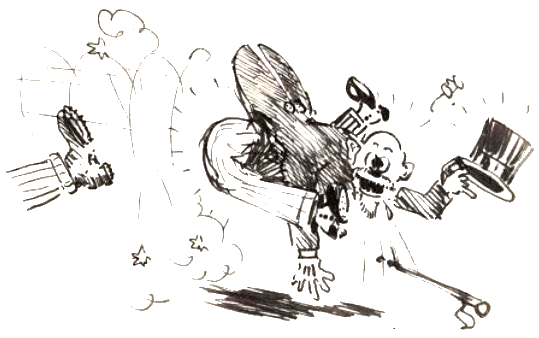
\includegraphics[width=1\textwidth]{images/brev75.png}
\end{center}

\breakpage